\section{Runtime Application Tuning} \label{rat}

Once the DTA analysis is finished and the Tuning Model (TM) has been generated, the optimized application can be used in production. 

READEX targets to exploit the dynamically changing requirements of the application to save energy consumed during the application production run. In order to fulfill this requirement of exploiting dynamism, system configuration switching is done at runtime. This dynamic switching of tuning parameters is applied during the Runtime Application Tuning (RAT) phase of READEX by the low-overhead READEX Runtime Library (RRL). 

RRL is implemeted as a Score-P Substrate Plugin using the Substrate Plugin Interface \cite{Schoene2017}. This plugin interface allows for generic access to measurement data at runtime without direct integration into Score-P. This approach acts to reduce maintenance and integration efforts by keeping the RRL as a separate entity. As a substrate plugin, the RRL has
access to all measurement data gathered through various means of instrumentation and uses this information to make switching decisions based on the tuning model created at design time.

RRL implements three main mechanisms in order to apply the dynamic configuration switching at runtime; namely scenario detection, configuration switching and calibration. This section contains the details of the first two mechanisms whereas the calibration mechanism is presented in detail in Section \ref{sec:calibration}.
Figure~\ref{fig:rrl} shows the detailed architecture of RRL, and will be used to explain the three mechnaism mentioned above.

\begin{figure}[!t]
\centering
%\includegraphics[trim={7cm 2cm 5.5cm 2cm},clip,width=3in]{readex-approach}
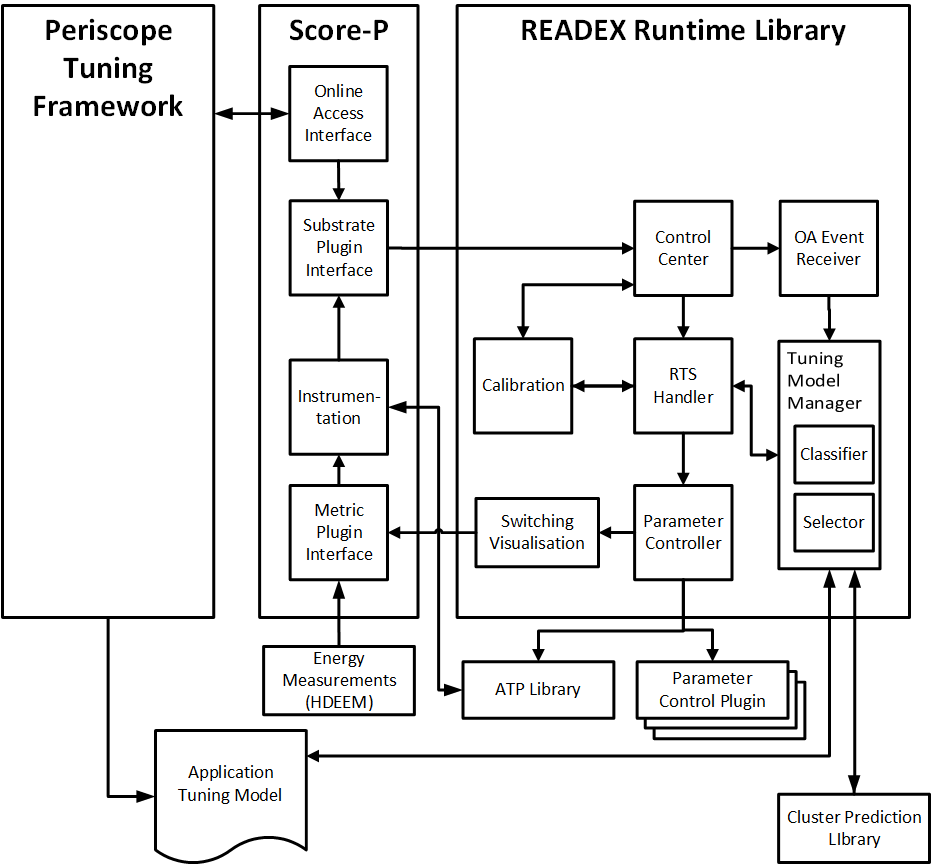
\includegraphics[width=.95\columnwidth]{figures/RRL_Architecture.png}
\caption{Architecture of the READEX Runtime Library (RRL)}
\label{fig:rrl}
\end{figure}

\paragraph{Scenario Detection}: Runtime detection of the upcoming scenario is a process that involves several modules in
the RRL architecture depicted in Figure~\ref{fig:rrl}. Upon approaching a new region, Control Center receives notification from Score-P. The Control Center registers the new region with the Tuning Model Manger (TMM). Different event notifications received by Control Center from Score-P are forwarded to RTS Handler and Calibration. These events include \textit{region enter, region exit} and \textit{user parameter}. The RTS Handler maintains the current call stack and collects the additional identifiers. Additional identifiers are specified in the application by annotating them as user parameters, which are passed by Score-P to the RTS Handler via the Control Center as user parameter events. Upon receiving an enter region notification from Score-P during the application run,
the RTS Handler checks with the Tuning Model Manager (TMM) whether the current region is a significant or an unknown region through the is significant function. If it is an unknown region, the calibration mechanism is invoked.
If the region is significant, the RTS Handler first requests for the number of additional identifiers. Once the required number of additional identifiers are collected by RTS Handler through \textit{user parameter} event notifications, the current rts is identified by both the call stack and the additional identifires. RTS Handler then requests a new configuration for rthe current rts from the Tuning Model Manager which is
then passed to the Parameter Controller by RTS handler to apply the configuration switching. 
\paragraph{Configuration Switching}: Switching of parameter settings is performed through the parameter control plugins that are also employed during the DTA phase.
During scenario detection, if the region entered is detected to be significant by the RTS Handler, the RTS Handler gets a new configuration from the Tuning Model Manager for
the generated rts. This configuration is passed to the Parameter
Controller, which sets the configuration through the respective Parameter Control Plugins (PCP).

Upon receiving an exit region event, the RTS Hander checks if the current region was set up for calibration. If yes, it requests the configuration for the currently exited region from the
Calibration module. Once the RTS handler gets back the configuration from the calibration module, it passes this configuration to the TMM which stores the new configuration for the respective rts. If the region was not set up for calibration, then the Parameter Controller is informed that it might want to unset the current configuration. 

The Parameter Controller supports two different modes: \textit{reset} and \textit{no-reset}. The first mode maintains a configuration stack. Whenever a new configuration is set, the previous configuration is pushed onto this stack. When the corresponding unset occurs, the element is removed from the stack and the previous configuration is set. If the no-reset mode is selected, the current configuration stays active until a new configuration is set. The unset is ignored. This behaviour is configurable by the user. By default, \textit{reset} mode is enabled.

\paragraph{Calibration}: For the already seen scenarios, RRL extracts the optimal configuration directly from the TM. For the un-seen ones an RRL calibration mechanism \ref{sec:calibration} is used to find the optimal system configuration based on machine learning algorithms and the data stored in the tuning model. 

 